%!TEX root = ../GLM_Becerra_Lopez.tex

\section{Resultados}
\label{sec:resultados}

En las figuras \ref{fig:comp_pooling_resids}, \ref{fig:no_pooling_resids} y \ref{fig:three_levels_resids} se muestran para cada uno de los modelos, los residuales en el eje $y$ y en el eje $x$ se muestra el índice de la observación, donde las observaciones están ordenadas de acuerdo a código postal. En el modelo de unidades iguales es evidente un patrón, que viene de la correlación entre las observaciones que existe dentro de cada código postal. En el modelo de unidades independientes los patrones del código postal ya no son tan evidentes como en el modelo de unidades iguales. Lo mismo pasa con el modelo multinivel, ya no hay un patrón evidente.

\begin{figure}[H]
    \centering
    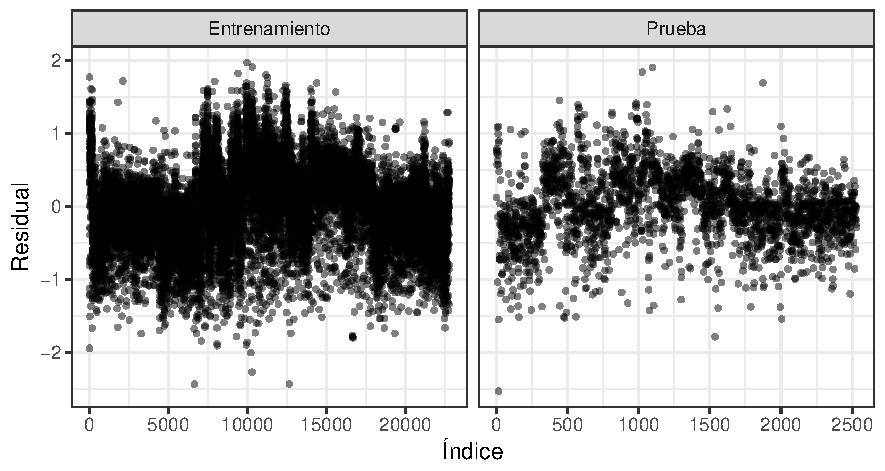
\includegraphics[width=0.7\textwidth]{images/comp_pooling_resids.pdf}
    \caption{Residuales de modelo de unidades iguales}
    \label{fig:comp_pooling_resids}
\end{figure}

\begin{figure}[H]
    \centering
    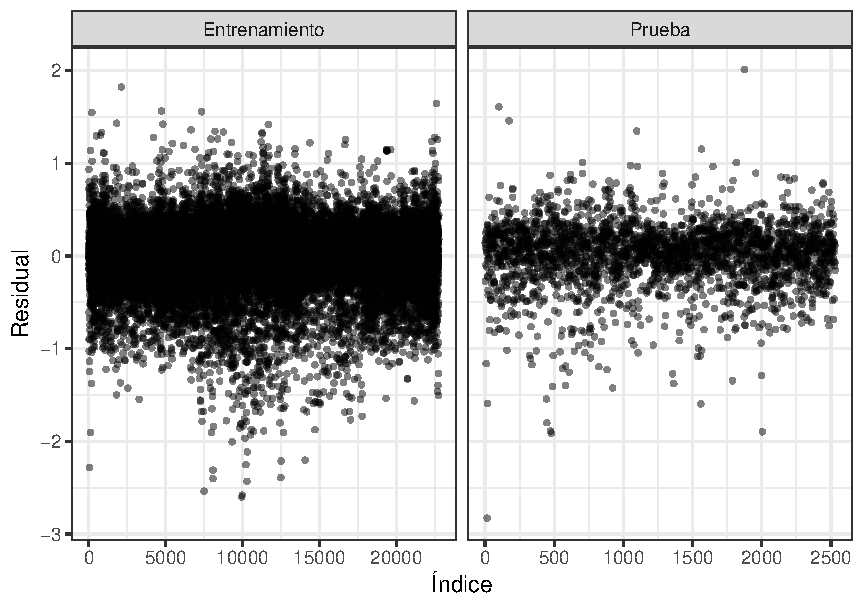
\includegraphics[width=0.7\textwidth]{images/no_pooling_resids.pdf}
    \caption{Residuales de modelo de unidades independientes}
    \label{fig:no_pooling_resids}
\end{figure}

\begin{figure}[H]
    \centering
    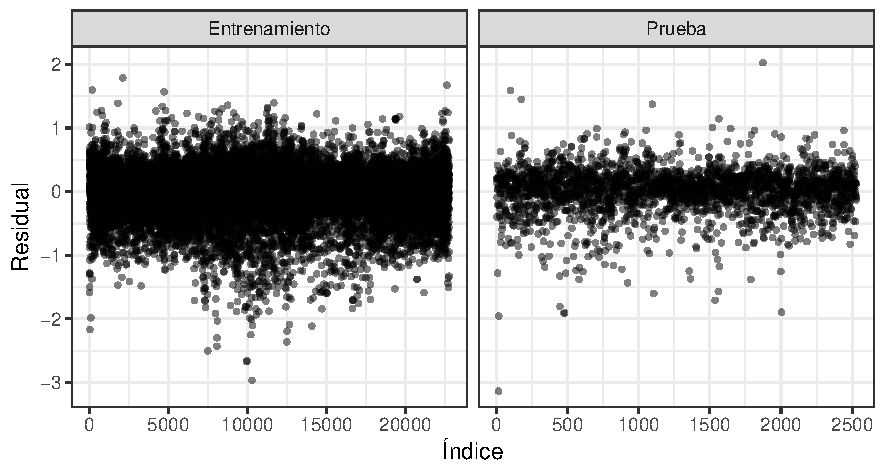
\includegraphics[width=0.7\textwidth]{images/three_levels_resids.pdf}
    \caption{Residuales de modelo multinivel}
    \label{fig:three_levels_resids}
\end{figure}

En las figuras \ref{fig:comp_pooling_obs_vs_pred}, \ref{fig:no_pooling_obs_vs_pred} y \ref{fig:three_levels_obs_vs_pred} se puede ver para cada observación el valor observado contra el valor ajustado de cada modelo. En todos se aprecia una varianza considerablemente grande; y en el modelo de unidades iguales, el modelo tiende a sobreestimar los valores pequeños, mientras que en valores grandes pasa lo contrario. Este efecto persiste, pero en mucho menor medida, en los otros dos modelos.

\begin{figure}[H]
    \centering
    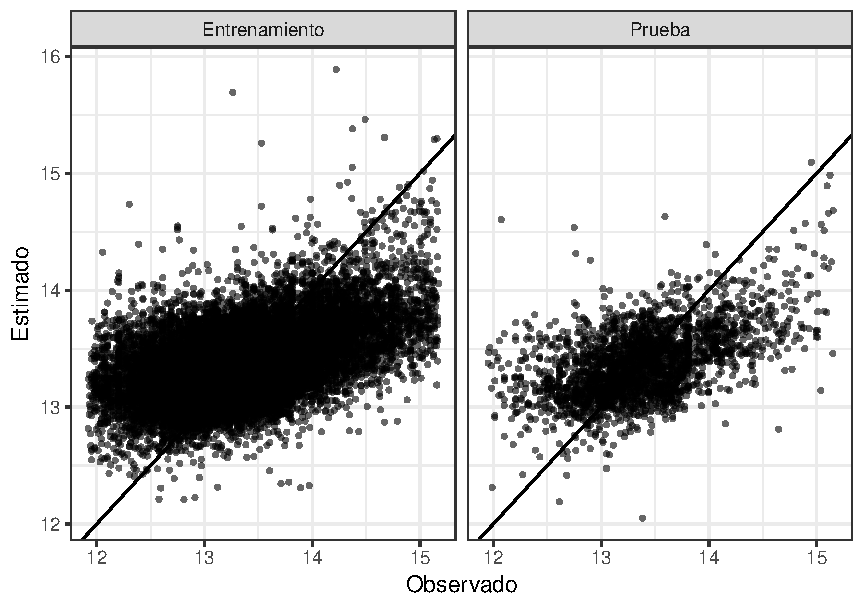
\includegraphics[width=0.7\textwidth]{images/comp_pooling_obs_vs_pred.pdf}
    \caption{Ajustado contra observado en modelo de unidades iguales}
    \label{fig:comp_pooling_obs_vs_pred}
\end{figure}

\begin{figure}[H]
    \centering
    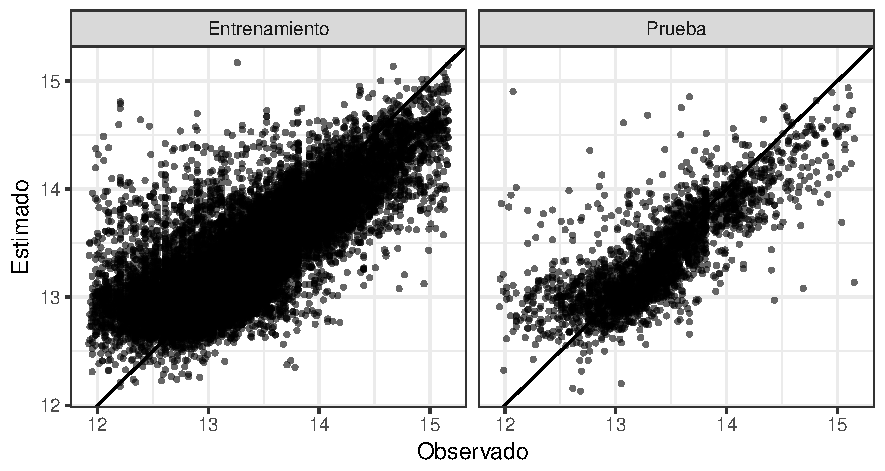
\includegraphics[width=0.7\textwidth]{images/no_pooling_obs_vs_pred.pdf}
    \caption{Valor ajustado contra observado en modelo de unidades independientes}
    \label{fig:no_pooling_obs_vs_pred}
\end{figure}


\begin{figure}[H]
    \centering
    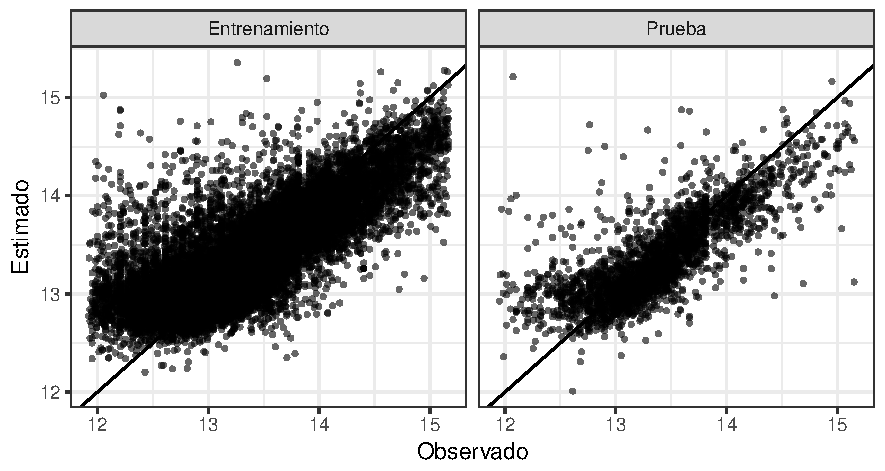
\includegraphics[width=0.7\textwidth]{images/three_levels_obs_vs_pred.pdf}
    \caption{Valor ajustado contra observado en modelo multinivel}
    \label{fig:three_levels_obs_vs_pred}
\end{figure}

En las figuras \ref{fig:no_pooling_param_values} y \ref{fig:three_levels_param_values} se muestran los valores de los parámetros junto con sus intervalos al 95\% de probabilidad del modelo de unidades independientes y del modelo multinivel. En el modelo de unidades independientes hay varios parámetros que tienen una varianza muy grande, y hay incluso algunos códigos postales que tienen un parámetro de pendiente negativo, lo cual intuitivamente no hace mucho sentido, pues eso significaría que a menor tamaño, la casa es más grande; pero recordando el análisis exploratorio, estas estimaciones negativas corresponden a los códigos postales con pocas observaciones en las cuales se podía apreciar una tendencia negativa; pero esto no es nada más que ruido de la muestra pequeña que se tiene. En el modelo multinivel, al tomar fuerzas de los hiperparámetros, no se tienen estimaciones puntuales negativas, y los intervalos de probabilidad son mucho más pequeños; sin embargo, sí se aprecia cambio entre los parámetros; es decir, el modelo está captando las diferencias de precio que existen entre los códigos postales.

\begin{figure}[H]
    \centering
    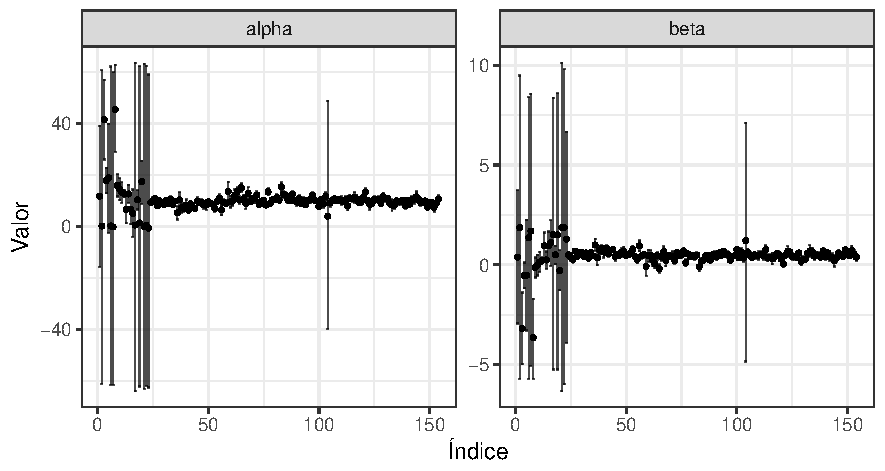
\includegraphics[width=0.7\textwidth]{images/no_pooling_param_values.pdf}
    \caption{Valor e intervalos de probabilidad de parámetros de modelo de unidades independientes}
    \label{fig:no_pooling_param_values}
\end{figure}

\begin{figure}[H]
    \centering
    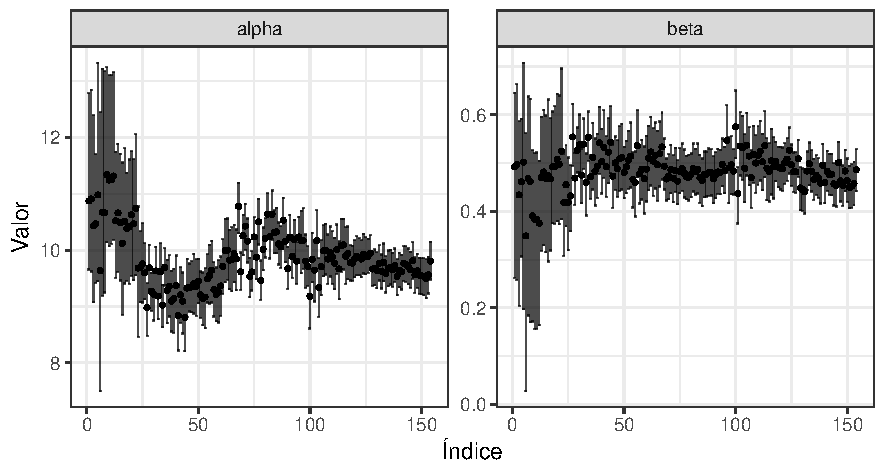
\includegraphics[width=0.7\textwidth]{images/three_levels_param_values.pdf}
    \caption{Valor e intervalos de probabilidad de parámetros de modelo multinivel}
    \label{fig:three_levels_param_values}
\end{figure}

Para observar el efecto de las diferencias en los parámetros, en las figuras \ref{fig:no_pooling_obs_vs_pred_train_by_neighborhood_zip_regression_lines} y \ref{fig:three_levels_obs_vs_pred_train_by_neighborhood_zip_regression_lines} se muestran las pendientes de regresión de código postal de cada modelo. Cada figura tiene muchas subgráficas, cada una representando un vecindario. Dentro de cada subgráfica se muestran los puntos de las ventas y además las líneas de regresión ajustadas a cada código postal dentro de cada vecindario. Se puede ver que en el modelo de unidades independientes cambian mucho las líneas, sobre todo en los vecindarios en los que hay pocos datos, llegando a haber líneas con pendientes negativas, lo cual no tiene mucho sentido dado el contexto del problema. El modelo nivel muestra pendientes más estables, y sobre todo, en los vecindarios y códigos postales, se mantiene siempre la pendiente positiva.

\begin{figure}[H]
    \centering
    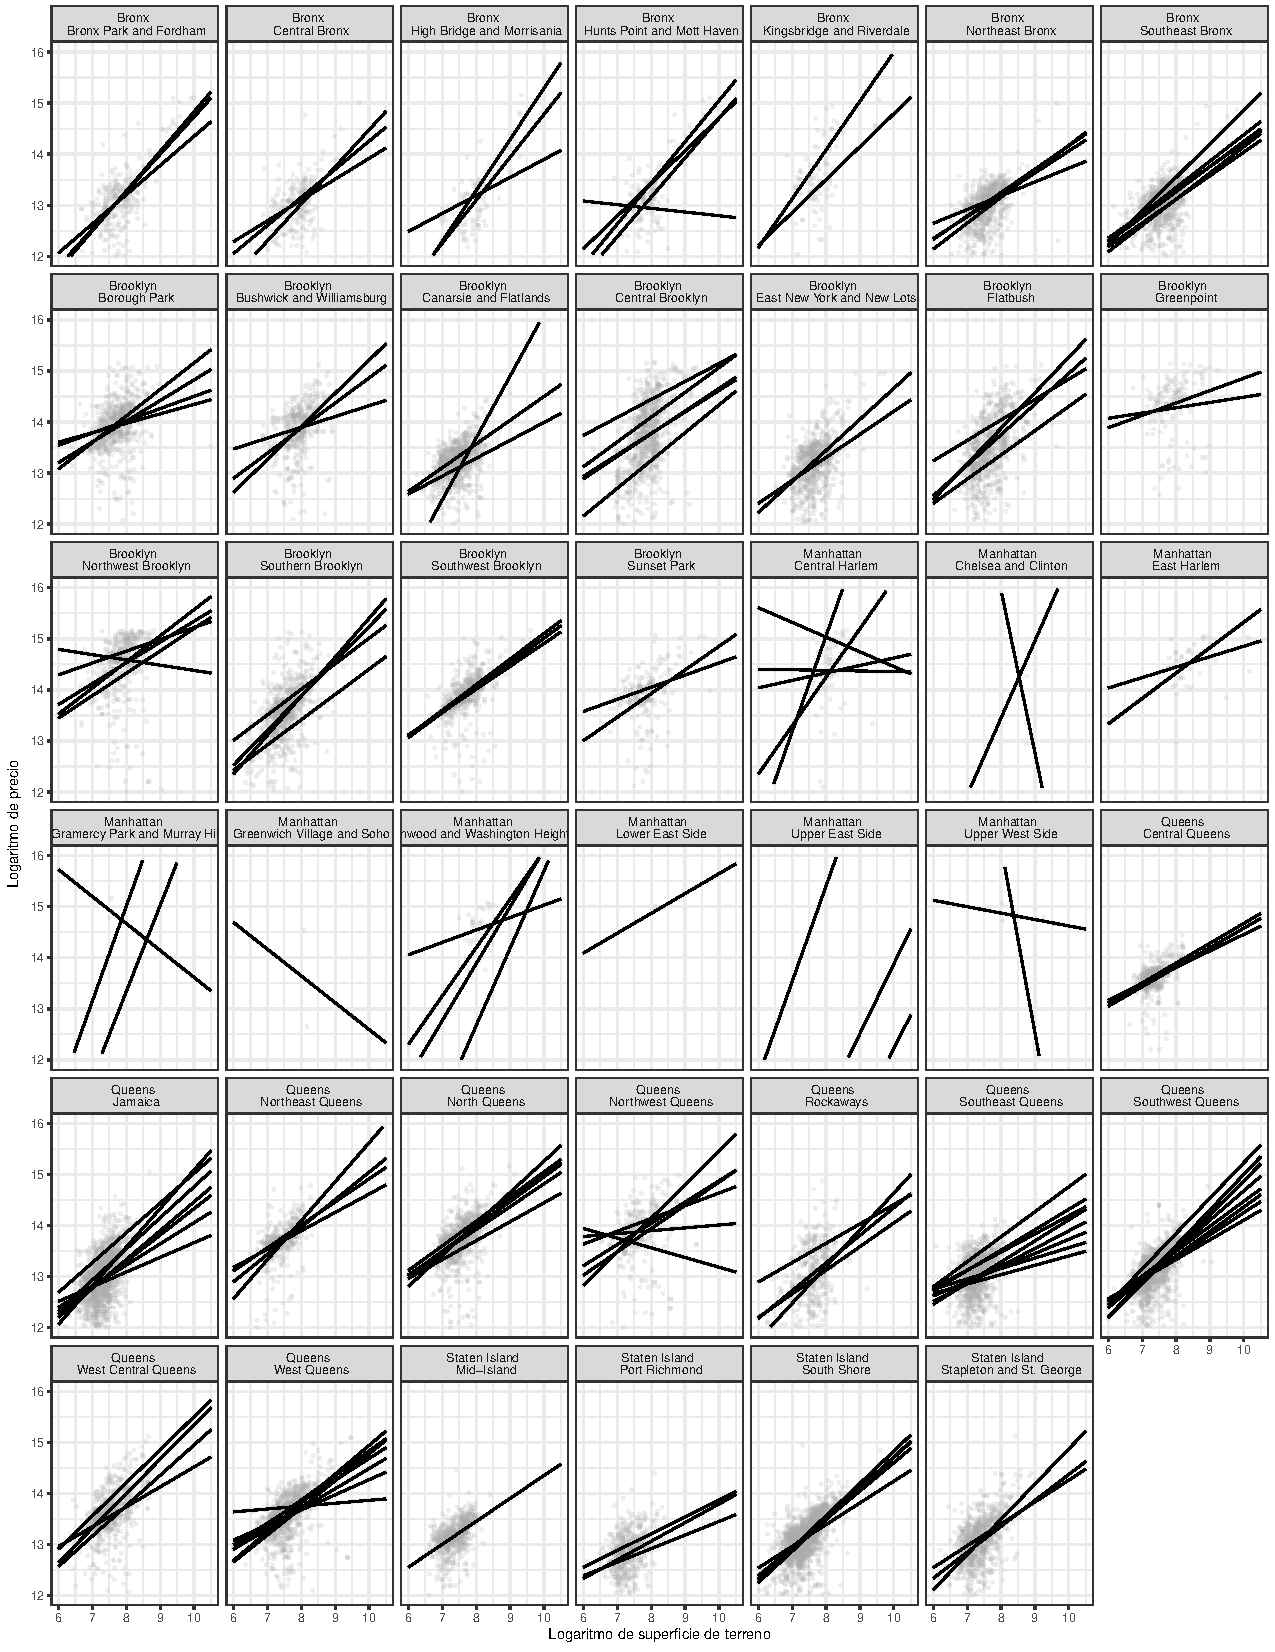
\includegraphics[width=\textwidth]{images/no_pooling_obs_vs_pred_train_by_neighborhood_zip_regression_lines.pdf}
    \caption{Modelo de unidades independientes: Diagramas de dispersión de logaritmo de superficie de terreno contra logaritmo del precio, separados por vecindario. Dentro de cada gráfica de vecindario, se muestran las líneas de regresión de cada código postal.}
    \label{fig:no_pooling_obs_vs_pred_train_by_neighborhood_zip_regression_lines}
\end{figure}

\begin{figure}[H]
    \centering
    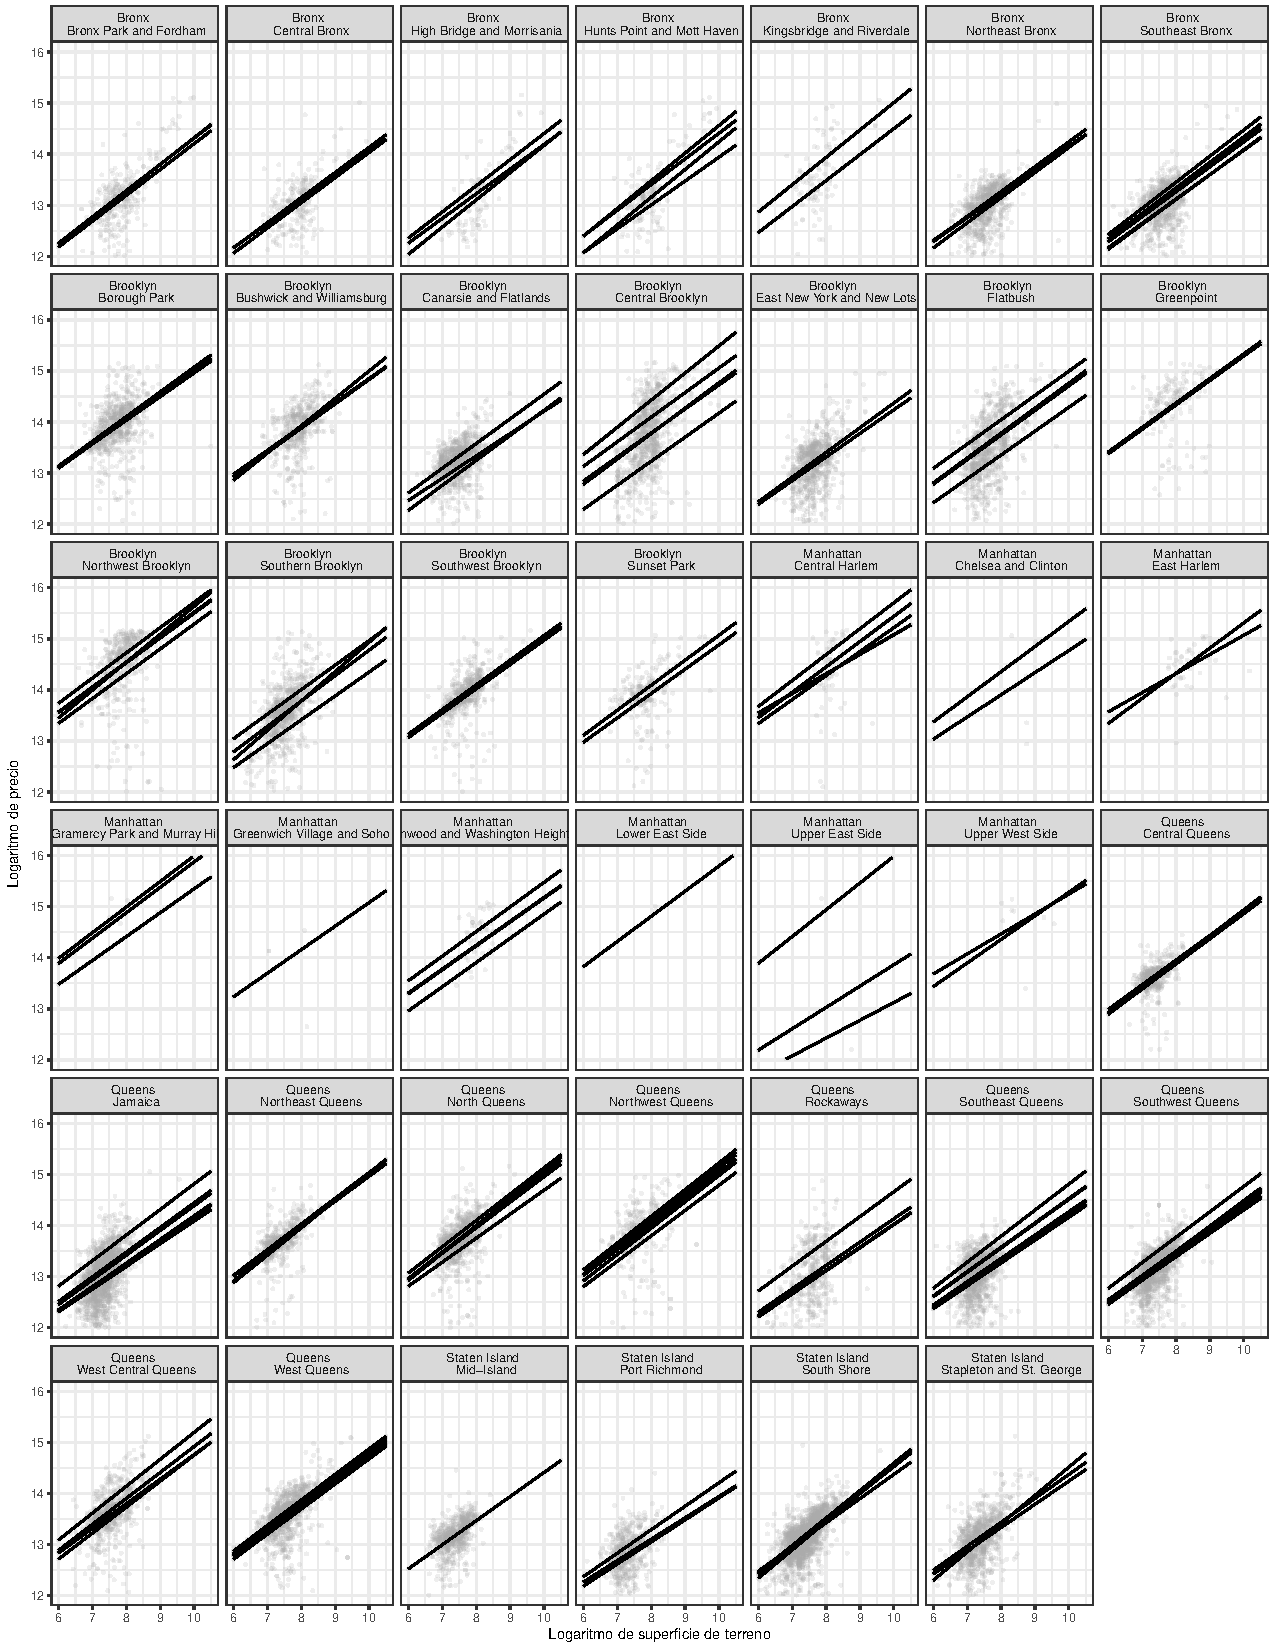
\includegraphics[width=\textwidth]{images/three_levels_obs_vs_pred_train_by_neighborhood_zip_regression_lines.pdf}
    \caption{Modelo multinivel: Diagramas de dispersión de logaritmo de superficie de terreno contra logaritmo del precio, separados por vecindario. Dentro de cada gráfica de vecindario, se muestran las líneas de regresión de cada código postal.}
    \label{fig:three_levels_obs_vs_pred_train_by_neighborhood_zip_regression_lines}
\end{figure}


Para medir el desempeño de los distintos modelos, se pueden usar distintas medidas. En este trabajo, se utilizan tres: el DIC (\textit{Deviance Information Criterion}), la raíz del error cuadrático medio (RMSE) y el error medio absoluto (MAE). Para las tres medidas, es preferible tener un menor valor. En la tabla \ref{tab:dic_rmse_mae} se muestran los valores de estas medidas para cada uno de los modelos. El modelo de unidades iguales es claramente inferior, pues los valores son mucho mayores. Entre el modelo de unidades independientes y el multinivel hay competencia, pues el primero tiene mayor DIC pero menores MAE y RMSE. Sin embargo, las diferencias en MAE y RMSE no son muy grandes; y además, viendo los resultados anteriores, el modelo multinivel es más robusto que el de unidades independientes.

\begin{table}[]
	\centering
	\caption{Valores de DIC, RMSE y MAE de cada modelo.}
	\label{tab:dic_rmse_mae}
	\begin{tabular}{|l|c|c|c|c|c|}
	\hline
	                        &           & \multicolumn{2}{c|}{Entrenamiento} & \multicolumn{2}{c|}{Prueba} \\ \hline
	                        & DIC       & MAE              & RMSE            & MAE          & RMSE         \\ \hline
	Unidades iguales        & 630,996   & 287,374          & 461,166         & 283,847      & 446,443      \\ \hline
	Unidades independientes & 7,239,403 & 188,123          & 315,006         & 190,248      & 324,864      \\ \hline
	Multinivel              & 16,716    & 191,383          & 324,493         & 192,564      & 335,204      \\ \hline
	\end{tabular}
\end{table}

% > readRDS("../out/models/model_comp_pooling.rds")$BUGSoutput$DIC
% [1] 630996.6
% > readRDS("../out/models/model_no_pooling.rds")$BUGSoutput$DIC
% [1] 7239403
% > readRDS("../out/models/model_three_levels.rds")$BUGSoutput$DIC
% [1] 16716.46

% > (mae_train_comp_pooling <- mean(abs(preds_comp_pooling$res)))
% [1] 287374.6
% > (mae_test_comp_pooling <- mean(abs(preds_test_comp_pooling$res)))
% [1] 283847
% > (mae_train_no_pooling <- mean(abs(preds_no_pooling$res)))
% [1] 188123.9
% > (mae_test_no_pooling <- mean(abs(preds_test_no_pooling$res)))
% [1] 190248.7
% > (mae_train_three_levels <- mean(abs(preds_three_levels$res)))
% [1] 191383.7
% > (mae_test_three_levels <- mean(abs(preds_test_three_levels$res)))
% [1] 192564

% > (rmse_train_comp_pooling <- sqrt(mean(preds_comp_pooling$res^2)))
% [1] 461166.2
% > (rmse_test_comp_pooling <- sqrt(mean(preds_test_comp_pooling$res^2)))
% [1] 446443.7
% > # RMSEs
% > (rmse_train_no_pooling <- sqrt(mean(preds_no_pooling$res^2)))
% [1] 315006.2
% > (rmse_test_no_pooling <- sqrt(mean(preds_test_no_pooling$res^2)))
% [1] 324864.2
% > # RMSEs
% > (rmse_train_three_levels <- sqrt(mean(preds_three_levels$res^2)))
% [1] 324493.5
% > (rmse_test_three_levels <- sqrt(mean(preds_test_three_levels$res^2)))
% [1] 335204.5

